This chapter aims to put this report in context by providing a brief overview of some of the central concepts of the \Gls{barricelli} computer.

\section{MIMD Computing}

\Gls{barricelli}, the solution computer presented in this report, is a \Gls{MIMD} computer. \Gls{MIMD}, or Multiple Instruction, Multiple Data, is a class of computer architectures involving multiple autonomous computing units executing different instructions on different data.
Thus, a MIMD computer system consists of several fully independent processing units or cores, interconnected in some way.
Each core/processor is able to work fully independently and asynchronously with their counterparts.
Because of this MIMD lends itself quite well to high performance computing through parallelism.

Communication between the different, possibly hetereogeneous independant computing units is either done by message passing, or sharing memory between processors.
Computers that solve communication using message passing might not have any shared memory between the processing units at all.
Each processing unit instead holds its own private memory.
This is called a distributed memory model.
Most MIMD computers implement some hybrid memory solution using both shared memory and distributed memory.

A simplified block-level overview of a MIMD computer can be seen in figure \vref{figure:mimd-block-diagram}.
The computer in the figure uses a shared memory model.
In the figure, the blocks labeled PU are induvidual processing units.

\begin{figure}[H]
\begin{center}
    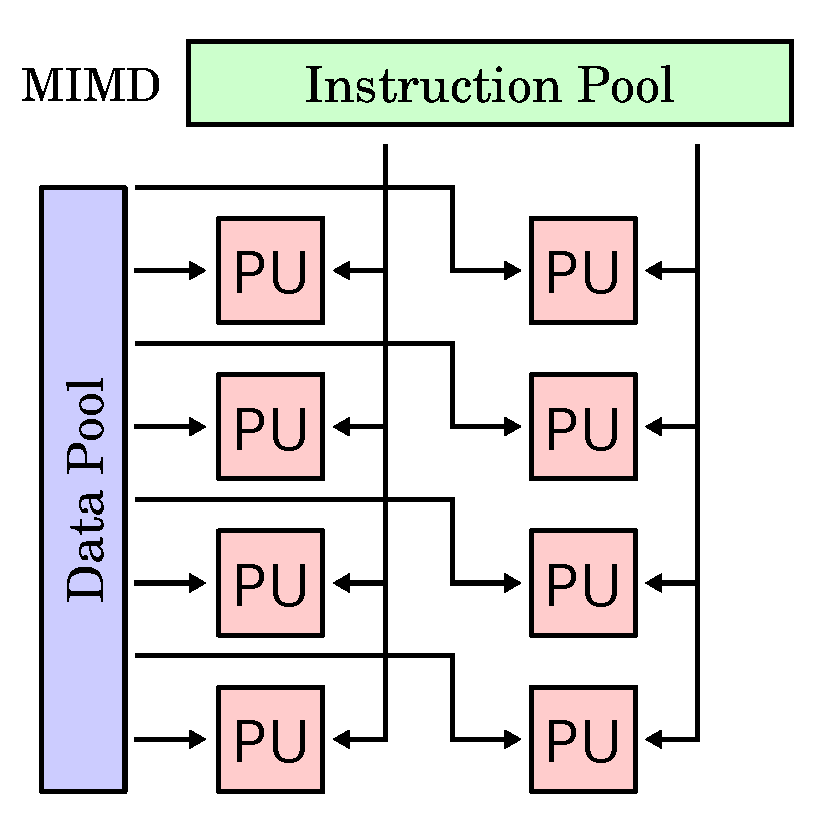
\includegraphics[width=\textwidth/2]{fig/mimd-block-diagram.pdf}
    \label{figure:mimd-block-diagram}
    \caption[
    Block-level overview of a MIMD computer with a shared memory model
    ]{
    Block-level overview of a MIMD computer with a shared memory model\footnote{http://en.wikipedia.org/wiki/File:MIMD.svg}}
\end{center}
\end{figure}

MIMD architecture forms the basis in the great majority all today’s multi-core superscalar processors.
This is in contrast to the early uniprocessors, which were based on SISD, or Single Instruction stream, Single Data stream. 


Examples of well-known MIMD computing platforms today include Intel's Larrabee platform, and computer clusters connected for instance over the internet.

\section{Genetic Algorithms}

A genetic algorithm is a specific type of heuristic search algorithm that is very useful for finding approximate solutions to hard optimization and search problems.
A hard problem in this context is a problem for which there exists no algorithm for feasibly computing a solution within a reasonable amount of time.
In practice, this typically means NP-hard problems.
Classical examples of hard problems for which genetic algorithms can find suitible approximations include the Satisfiability Problem, the Traveling Salesman Problem and the Binary Knapsack Problem, to name a few.
Efficiently finding good approximations to this class of problems is extremely important for many heavy instrustry processes such as planning and scheduling of processes, finding optimal placement and routing of components in microchip manufacturing, and many other business-critical tasks.

The distringuising feature of a genetic algorithm compared to other heuristic search algorithms is how it performs its search: it mimics the natural process of evolution to find fit approximations in the search space.
A genetic algorithm represents possible solutions to a given problem as individuals of a population.
The individuals' fitness is calculated by a problem-specific fitness function, and fit individuals are combined together to create new individuals, mimicing the process of natural selection.
The idea is that after simulating a number of virtual generations of individuals, the fittest individual will have survived, and provides a good approximation to the solution.

\subsection{Concepts and Definitions}

To fully understand the inner workings of the \Gls{barricelli}, it is useful to become aquainted with the basic concepts of genetic algorithms.
This subsection of the document defines some genetic algorithm concepts that are used elsewhere in the report.

\paragraph{Individual}
An individual is one possible solution to a given problem.

\paragraph{Population}
A population is the group of all current individuals in a given experiment.

\paragraph{Fitness}
The fitness value of an individual is an evaluation of how close it is to the theoretically perfect individual. It is calculated by an objective rating function.

\paragraph{Selection}
Probabilistic selection of rated individuals allowed to reproduce.
The probability of picking a certain individual is normally proportional to its fitness rating.

\paragraph{Crossover}
Reproduction method involving combining individuals in some way to form a new individual (problem specific). 

\paragraph{Mutation}
Mutation of an individual. It is either random or based on specific rules (problem specific). 

\subsection{Pseudo-code for a General Genetic Algorithm}

Algorithm \vref{algorithm:pseudo-code-for-ga} shows example pseudo code for a general genetic algorithm.

\begin{figure}[H]
\begin{algorithm}[H]
\SetAlgoLined
\DontPrintSemicolon
\KwData{A population of random individuals}
\KwResult{A quite fit individual}
\Begin{
    $ k \longleftarrow 0 $\;
    $ P_k \longleftarrow $ a population of $ n $ randomly-generated individuals\;
    Compute $fitness(i)$ for each $ i \in P_k $\;
    \While{$ max(fitness(i) \in P_k) < threshold and k < maxIterations $}{
        Selection:\;
        Select $ (1 - x_i) \times n $ members of $ P_k $ and insert them into $ P_{k + 1} $\;

        Crossover:\;
        Select $ x_i \times n $ members of $ P_k $, pair them up, produce offspring, insert offspring into $ P_k $\;


        Mutation:\;
        Mutate $ \mu \times n $ members of $ P_{k + 1} $\;
        Compute $ fitness(i) $ for each $ i \in P_k $\;
        $k \longleftarrow k + 1 $
    }
    \Return{the fittest individual in $ P_k $}
}
\caption{Generic genetic algorithm}
\label{algorithm:pseudo-code-for-ga}
\end{algorithm}
\end{figure}

\todo{tidy}

\subsection{Generational Genetic Algorithms}

Traditionally, genetic algorithms are implemented generationally \TODO{TODO: cite hromcovic or something}. That means that an entire population of individuals are rated and combined to create a completely new population, and the old population is discarded. The generational genetic algorithm can be seen as performing five steps:


\begin{enumerate}
    \item Start with an initial population
    \item Calculate the fitness of each individual in the generation
    \item Selection
    \item Crossover
    \item Mutation  
\end{enumerate}

The initial population is normally made from randomly generated individuals.
The diversity ensures that it is possible for the generation to evolve towards a solution without getting stuck in an early local maxima.
In the next stage the fitness of each individual calculated, which is very specific for the problem at hand.
If this fitness values exceeds some specified threshold, the solution is deemed good enough and the algorithm stops.
Note that it will not always finding a perfect solution, but one that is sufficient for the problem at hand.
If however none of the individuals end up with a fitness value above the threshold, the algorithm continues.

The solution is found during several phases though a selection, crossover and a mutation phase. 
These phases are used to evolve the population through several generations until an appropriate solution is found. 

The selection core aim to chose individuals for reproduction based on their fitness score.The selection is constructed in such that higher fitness score equals higher probability of being chosen. This does not necessary mean that only the fittest individuals are allowed to reproduce. An important concept of the genetic algorithm is to achieve diversity while exploring the different solutions. Diversity is important to prevent the algorithm from reaching what is known as a local maximum. E.g stage where it is unable to evolve any further even though the solution found is far from being optimal.

The crossover core uses the individuals from the selection to cross the individuals to produce new individuals. Because of the initial diversity in the initial population, this will cause the diversity to be large in the beginning. However this will settle in further generations. The goal of the crossover phase is to converge against a solution by continuos creating better a better generation of individuals. There are several methods for achieving the crossover of individuals, however, the different methods will not be discussed in great detail here. The different algorithms are highly dependent on the task at hand. However, the different crossover methods implemented in the employed in the galapagos architecture will be discussed in greater detail in section \vref{fpga:subsection:genetic_pipeline}.

However as an precaution, the individuals are passed through yet another phase, mutation. The goal of the mutation state is ensure diversity by mutating the individuals by some probability. The mutation process is usually a simple one by just modifying some of the bits in the individual. As with the crossover method, algorithms also exist for performing the mutation. 

Lastly, it is important to mention that there exist a lot of different classes of genetic algorithms. They usually use employ many different techniques for performing selection, crossover and mutation. The point of this project is not covering all of them. Actually, only a subset of problems will be supported on galapagos architecture. 


\todo{Fix this section}


\subsection{Continuous Genetic Algorithms}

A new and better strategy is gaining traction in the literature.\TODO{TODO: find a citation for this}.
Continuous genetic algorithms do away with the concept of discrete generations.
Rather, it continuously selects a few individuals, processes them, and returns them (or their offspring) to the population.
This erases the generational border, and is shown \TODO{TODO:cite our own research here, plus literature} to converge faster towards an optimal solution. This also implies that the operations involved in the genetic algorithm is  more easily parallelizeble, since the generation restriction no longer visible. More specific it allows the algorithm a possible way to work on both rated an unrated individuals on the same time. As the reader may have noticed in section, the algorithm presented were very sequential. 

This algorithm uses an other approach, by disregarding the generation boundaries. It is possible to both rate and handle rated elements simultaneously without bothering about generating specific generations of individuals that are passed to the next stage. The previous algorithm finished with one generation before start working on the next one. The continuous approach, work on individuals instead. E.g the individuals are continuously rated and passed along to reproduce. The same steps are performed, however, not in sequential order any more. All the steps has the possibility to be performed in parallel. This has the advantage of increasing the throughput. The problem is also more suited on MIMD architecture, like the one galapagos is based on.      





The genetic algorithm used in the Barricelli computer is a continuous genetic algorithm.


